\documentclass[a4paper,11pt]{article}
\usepackage{geometry}
\geometry{
    left=20mm,
    right=20mm,
    top=22mm,
    bottom=22mm,
    footskip=12mm
}

\usepackage{fontspec}
\setmainfont{Times New Roman}
\setmonofont[Scale=0.9]{Consolas}

\usepackage[russian]{babel}
\usepackage{amsmath,amssymb,amsfonts}
\usepackage{graphicx}
\graphicspath{{../../src/}{../../src/figures/}{../src/}{../src/figures/}{../../}{../}{./}}
\usepackage{booktabs}
\usepackage{tabularx}
\usepackage{xcolor}
\usepackage{titlesec}
\usepackage{caption}
\usepackage{subcaption}
\usepackage{tcolorbox}
\usepackage{hyperref}

\hypersetup{
    colorlinks=true,
    linkcolor=blue!70!black,
    citecolor=blue!70!black,
    urlcolor=teal!70!black,
    pdftitle={Теория динамической дифракции RCWA, 2D/3D угловое картирование флуоресценции GIXRF и резонансные линии Рэлея},
    pdfauthor={Antigravity AI},
    pdfsubject={RCWA, Near-field, Sherman equation, GIXRF, Rayleigh anomalies, 3D nanocolumns, FEM comparison}
}

% Цветовая гамма
\definecolor{primary}{RGB}{16, 54, 98}
\definecolor{secondary}{RGB}{35, 95, 145}
\definecolor{accent}{RGB}{180, 50, 40}

\titleformat{\section}{\color{primary}\normalfont\Large\bfseries}{\thesection}{1em}{}
\titleformat{\subsection}{\color{secondary}\normalfont\large\bfseries}{\thesubsection}{1em}{}
\titleformat{\subsubsection}{\color{black}\normalfont\normalsize\bfseries}{\thesubsubsection}{1em}{}

% Стилизованные блоки
\newtcolorbox{mathbox}[1][Формула]{
    colback=blue!3!white,
    colframe=primary!80!black,
    coltitle=white,
    arc=2mm,
    boxrule=0.8pt,
    left=3mm, right=3mm, top=2.5mm, bottom=2.5mm,
    title={#1},
    fonttitle=\bfseries
}

\newtcolorbox{remarkbox}[1][Замечание]{
    colback=yellow!6!white,
    colframe=orange!75!black,
    coltitle=white,
    arc=2mm,
    boxrule=0.8pt,
    left=3mm, right=3mm, top=2.5mm, bottom=2.5mm,
    title={#1},
    fonttitle=\bfseries
}

\begin{document}

\begin{titlepage}
    \centering
    \vspace*{1.2cm}
    
    {\Huge\bfseries\color{primary} Метод связанных волн (RCWA) и полуаналитический расчет рентгеновской флуоресценции (GIXRF) на периодических наноструктурах\par}
    
    \vspace{1.2cm}
    {\Large\bfseries Теория периодических решеток, кинематика резонансных линий Рэлея-Вуда, двумерные угловые карты и сравнение с FEM\par}
    
    \vspace{2.0cm}
    \begin{tcolorbox}[colback=blue!3!white,colframe=primary!70!black,arc=2mm,width=0.88\textwidth]
        \centering
        \textbf{Аннотация}\\[0.5em]
        \small Настоящий документ представляет собой строгое и всестороннее руководство по динамической теории дифракции рентгеновского излучения в приближении многих волн (Rigorous Coupled-Wave Analysis, RCWA / MBDDT) и её применению для моделирования выхода характеристической флуоресценции при скользящих углах падения (GIXRF). 
        
        В работе последовательно рассмотрены:
        1) вывод волнового уравнения и решение задачи на собственные значения в структурированном слое;
        2) численно стабильное удовлетворение граничных условий и восстановление ближнего поля;
        3) полуаналитический метод интегрирования уравнения Шермана через матричное произведение Адамара (Николаев, 2020);
        4) природа и строгий вывод кинематических резонансных линий дифракции Рэлея-Вуда на двумерных картах $(\phi, \alpha_i)$;
        5) детальный сравнительный анализ с методом конечных элементов (FEM, Soltwisch 2018, JCMwave).
    \end{tcolorbox}
    
    \vfill
    {\large 2026 г.\par}
\end{titlepage}

\tableofcontents
\newpage

\section*{Введение и физическая постановка задачи}
\addcontentsline{toc}{section}{Введение и физическая постановка задачи}

Рентгеновская флуоресценция при скользящих углах падения (\textit{Grazing-Incidence X-ray Fluorescence}, GIXRF) в сочетании с дифракцией и рефлектометрией (GIXD/XRR) является ведущим методом неразрушающего трехмерного нанометрового анализа полупроводниковых периодических структур, дифракционных решеток и массивов наноэлементов микроэлектроники \cite{soltwisch2018, nikolaev2020, dialameh2018}.

При облучении периодической наноструктуры коллимированным монохроматическим пучком рентгеновского излучения под скользящими углами $\alpha_i$ интерференция падающей и многократно дифрагированных волн формирует стоячую рентгеновскую волну (\textit{X-ray Standing Wave}, XSW). Локальная интенсивность поля возбуждает характеристическую флуоресценцию атомов материала.

Двумерное сканирование по двум углам — углу скольжения $\alpha_i$ и азимутальному углу поворота образца $\phi$ — порождает двумерные угловые карты интенсивности флуоресценции $Y(\phi, \alpha_i)$. На этих картах возникают характерные резонансные линии и осцилляционные узоры, содержащие исчерпывающую информацию о трехмерной геометрии наноструктуры (высоте, ширине, периоде, наклоне стенок и пространственном распределении легирующих элементов).

Документ состоит из 5 глав:
\begin{itemize}
    \item \textbf{Глава 1}: Уравнения Максвелла, скалярное приближение, геометрия решетки и спектральная задача на собственные значения.
    \item \textbf{Глава 2}: Граничные условия, численная устойчивость и точное восстановление 2D ближнего поля на плоскости.
    \item \textbf{Глава 3}: Полуаналитический расчет флуоресценции GIXRF по уравнению Шермана (матричная свертка Николаева, 2020).
    \item \textbf{Глава 4}: Двумерные угловые карты флуоресценции $(\phi, \alpha_i)$, природа резонансных линий Рэлея-Вуда и их теоретический вывод.
    \item \textbf{Глава 5}: Сравнительный анализ: полуаналитический RCWA против метода конечных элементов (FEM, Soltwisch 2018, JCMwave).
\end{itemize}

\newpage
\section{Уравнения Максвелла, геометрия решетки и задача на собственные значения}

\subsection{Уравнения Максвелла в рентгеновском диапазоне и скалярное приближение}

В классической электродинамике сплошных сред распространение монохроматического электромагнитного поля с гармонической временной зависимостью $e^{-i\omega t}$ описывается уравнениями Максвелла:
\begin{align}
    \nabla \times \mathbf{E} &= i \omega \mu_0 \mathbf{H}, \label{eq:maxwell_curlE} \\
    \nabla \times \mathbf{H} &= -i \omega \varepsilon_0 \varepsilon(\mathbf{r}) \mathbf{E}, \label{eq:maxwell_curlH} \\
    \nabla \cdot \big(\varepsilon(\mathbf{r}) \mathbf{E}\big) &= 0, \label{eq:maxwell_divE} \\
    \nabla \cdot \mathbf{H} &= 0. \label{eq:maxwell_divH}
\end{align}
Применяя оператор ротора к первому уравнению Максвелла (\ref{eq:maxwell_curlE}):
\begin{equation}
    \nabla \times (\nabla \times \mathbf{E}) = i \omega \mu_0 (\nabla \times \mathbf{H}).
\end{equation}
Подставляя второе уравнение Максвелла (\ref{eq:maxwell_curlH}) для $\nabla \times \mathbf{H}$:
\begin{equation}
    \nabla \times (\nabla \times \mathbf{E}) = i \omega \mu_0 \big(-i \omega \varepsilon_0 \varepsilon(\mathbf{r}) \mathbf{E}\big) = \omega^2 \mu_0 \varepsilon_0 \varepsilon(\mathbf{r}) \mathbf{E} = K^2 \varepsilon(\mathbf{r}) \mathbf{E},
\end{equation}
где $K = \omega / c = 2\pi / \lambda$ — волновое число излучения в вакууме ($c = 1/\sqrt{\mu_0 \varepsilon_0}$).

С другой стороны, раскрывая двойной ротор по известному векторному дифференциальному тождеству:
\begin{equation}
    \nabla \times (\nabla \times \mathbf{E}) = \nabla (\nabla \cdot \mathbf{E}) - \nabla^2 \mathbf{E}.
\end{equation}
Приравнивая оба выражения для $\nabla \times (\nabla \times \mathbf{E})$:
\begin{equation}
    \nabla (\nabla \cdot \mathbf{E}) - \nabla^2 \mathbf{E} = K^2 \varepsilon(\mathbf{r}) \mathbf{E} \implies \nabla^2 \mathbf{E} + K^2 \varepsilon(\mathbf{r}) \mathbf{E} - \nabla (\nabla \cdot \mathbf{E}) = 0.
    \label{eq:wave_intermediate}
\end{equation}

В неоднородной среде диэлектрическая проницаемость $\varepsilon(\mathbf{r})$ зависит от координат, поэтому дивергенция электрического поля $\nabla \cdot \mathbf{E} \neq 0$. Согласно третьему уравнению Максвелла (\ref{eq:maxwell_divE}) (закон Гаусса в отсутствие свободных зарядов), нулю равна дивергенция вектора электрического смещения $\mathbf{D} = \varepsilon_0 \varepsilon(\mathbf{r}) \mathbf{E}$:
\begin{equation}
    \nabla \cdot \big(\varepsilon(\mathbf{r}) \mathbf{E}\big) = 0.
\end{equation}
Раскрывая дивергенцию произведения скалярной функции $\varepsilon(\mathbf{r})$ на векторное поле $\mathbf{E}(\mathbf{r})$ по правилу Лейбница $\nabla \cdot (\phi \mathbf{A}) = \phi (\nabla \cdot \mathbf{A}) + \mathbf{A} \cdot \nabla \phi$:
\begin{equation}
    \varepsilon(\mathbf{r}) (\nabla \cdot \mathbf{E}) + \mathbf{E} \cdot \nabla \varepsilon(\mathbf{r}) = 0 \implies \nabla \cdot \mathbf{E} = - \mathbf{E} \cdot \frac{\nabla \varepsilon(\mathbf{r})}{\varepsilon(\mathbf{r})}.
\end{equation}
Подставляя найденное выражение для $\nabla \cdot \mathbf{E}$ в (\ref{eq:wave_intermediate}), с учетом минуса перед третьим слагаемым получаем точное \textbf{векторное волновое уравнение}:
\begin{equation}
    \nabla^2 \mathbf{E} + K^2 \varepsilon(\mathbf{r}) \mathbf{E} + \nabla \left( \mathbf{E} \cdot \frac{\nabla \varepsilon(\mathbf{r})}{\varepsilon(\mathbf{r})} \right) = 0.
    \label{eq:vector_wave_eq}
\end{equation}

\begin{mathbox}[Обоснование скалярного приближения в рентгеновской оптике]
В рентгеновском диапазоне длин волн ($\lambda \sim 0.1\dots 5$ нм) показатель преломления всех веществ чрезвычайно близок к единице:
\begin{equation}
    n(\mathbf{r}) = 1 - \delta(\mathbf{r}) + i \beta(\mathbf{r}), \quad \delta, \beta \sim 10^{-6}\dots 10^{-3} \ll 1.
\end{equation}
Диэлектрическая проницаемость среды равна $\varepsilon(\mathbf{r}) = n^2(\mathbf{r}) \approx 1 + \chi(\mathbf{r})$, где рентгеновская диэлектрическая восприимчивость равна:
\begin{equation}
    \chi(\mathbf{r}) = -2\delta(\mathbf{r}) + 2i\beta(\mathbf{r}), \quad |\chi(\mathbf{r})| \ll 1.
\end{equation}
Градиент диэлектрической проницаемости в третьем слагаемом уравнения (\ref{eq:vector_wave_eq}) имеет порядок:
\begin{equation}
    \frac{\nabla \varepsilon}{\varepsilon} = \frac{\nabla \chi}{1 + \chi} \approx \nabla \chi \sim O(10^{-4}).
\end{equation}
При малых углах скольжения ($\alpha_i \lesssim 5^\circ$) поляризационные эффекты пренебрежимо малы (поляризационный фактор $\cos(2\theta) \approx 1$). Поэтому слагаемым $\nabla(\mathbf{E} \cdot \nabla \varepsilon / \varepsilon)$ можно с высокой точностью пренебречь \cite{nikolaev2020, mikulik_rcwa}.
\end{mathbox}

Задача строго сводится к \textbf{скалярному уравнению Гельмгольца}:
\begin{equation}
    \nabla^2 E(\mathbf{r}) + K^2 \big(1 + \chi(\mathbf{r})\big) E(\mathbf{r}) = 0.
    \label{eq:helmholtz_scalar}
\end{equation}

\subsection{Геометрия периодической решетки и падающая волна}

Рассмотрим одномерно-периодическую решетку прямоугольного профиля (ламеллярная решетка, рис.~\ref{fig:geometry}):
\begin{itemize}
    \item Ось $x$ направлена перпендикулярно штрихам решетки вдоль направления периодичности (период $d$);
    \item Ось $y$ направлена вдоль штрихов (структура трансляционно-инвариантна вдоль $y$);
    \item Ось $z$ направлена вглубь структуры: $z < 0$ — вакуум, $0 \le z \le t$ — структурированный слой решетки толщиной $t$, $z > t$ — однородная подложка.
\end{itemize}
Ширина штриха составляет $w = \Gamma d$, где $\Gamma \in (0, 1)$ — коэффициент заполнения (\textit{duty cycle}). Восприимчивость материала штриха равна $\chi$, межштрихового пространства — $\chi_b$ (в вакууме $\chi_b = 0$), подложки — $\chi_{\text{sub}}$.

Направление падающей волны задается двумя углами:
\begin{itemize}
    \item $\alpha_i$ (или $\alpha$) — угол скольжения относительно плоскости поверхности $xy$;
    \item $\phi$ — азимутальный угол поворота образца относительно плоскости падения. Угол $\phi = 0^\circ$ соответствует конической геометрии (плоскость падения параллельна линиям решетки).
\end{itemize}

Волновой вектор падающей волны $\mathbf{K} = (K_x, K_y, K_z)$ имеет компоненты:
\begin{equation}
    K_x = K \cos\alpha_i \sin\phi, \quad K_y = K \cos\alpha_i \cos\phi, \quad K_z = K \sin\alpha_i.
    \label{eq:incident_k}
\end{equation}

\begin{figure}[htbp]
    \centering
    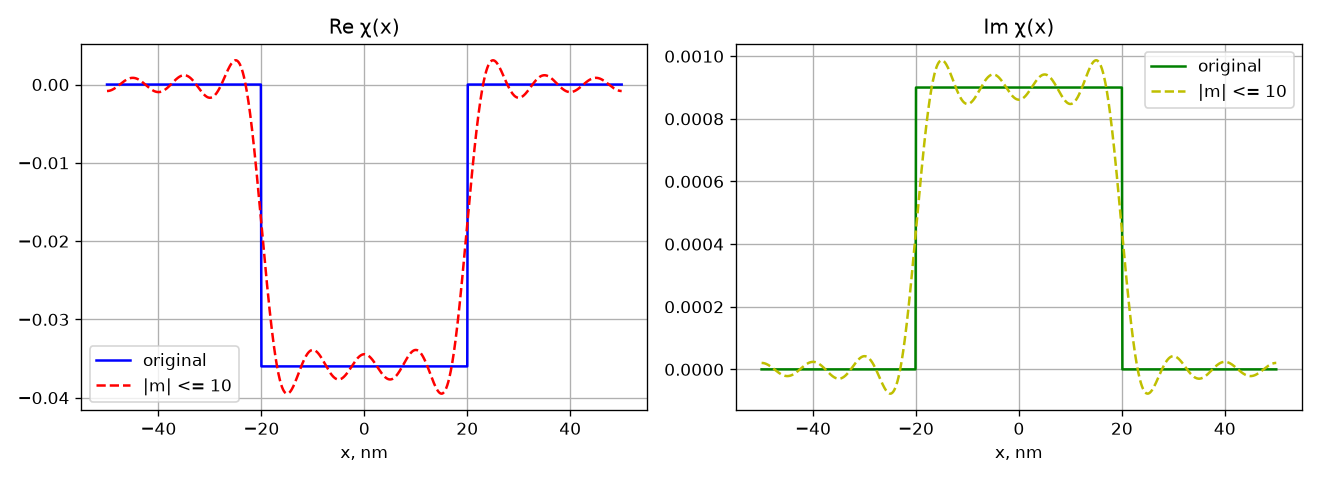
\includegraphics[width=0.85\textwidth]{figures/fourier.png}
    \caption{Пространственный профиль рентгеновской восприимчивости $\chi(x)$ периодической решетки и его спектральное разложение в ряд Фурье.}
    \label{fig:geometry}
\end{figure}

\subsection{Теорема Флоке-Блоха и разложение поля по пространственным гармоникам}

В силу теоремы Блоха-Флоке решение уравнения Гельмгольца (\ref{eq:helmholtz_scalar}) в периодической среде ищется в виде суммы пространственных гармоник:
\begin{equation}
    E(x, y, z) = e^{i K_y y} \sum_{h = -\infty}^{+\infty} E_h(z) e^{i k_{hx} x},
    \label{eq:bloch_field}
\end{equation}
где латеральный волновой вектор $h$-й гармоники равен:
\begin{equation}
    k_{hx} = K_x + \frac{2\pi h}{d}.
    \label{eq:khx}
\end{equation}
Квадрат полного продольного волнового вектора равен $k_{\parallel h}^2 = k_{hx}^2 + K_y^2$.

\subsection{Разложение восприимчивости в ряд Фурье}

Периодическая восприимчивость $\chi(x) = \chi(x + d)$ раскладывается в ряд Фурье:
\begin{equation}
    \chi(x) = \sum_{m = -\infty}^{+\infty} \chi_m e^{i \frac{2\pi m}{d} x}, \quad \chi_m = \frac{1}{d} \int_{-d/2}^{d/2} \chi(x) e^{-i \frac{2\pi m}{d} x} dx.
\end{equation}
Для прямоугольного штриха шириной $w = \Gamma d$, симметрично центрированного в $x = 0$:
\begin{mathbox}[Коэффициенты Фурье ламеллярной решетки]
\begin{equation}
    \chi_m = (\chi - \chi_b) \, \Gamma \, \operatorname{sinc}(m \Gamma) + \chi_b \, \delta_{m, 0},
    \label{eq:fourier_chi_analytic}
\end{equation}
где $\operatorname{sinc}(\xi) = \sin(\pi \xi) / (\pi \xi)$, а $\delta_{m,0}$ — символ Кронекера.
\end{mathbox}

\subsection{Дифференциальная система уравнений и матрица взаимодействия \texorpdfstring{$A$}{A}}

Раскроем вывод дифференциальной системы шаг за шагом. Скалярное уравнение Гельмгольца (\ref{eq:helmholtz_scalar}) в декартовых координатах имеет вид:
\begin{equation}
    \frac{\partial^2 E}{\partial x^2} + \frac{\partial^2 E}{\partial y^2} + \frac{\partial^2 E}{\partial z^2} + K^2 E + K^2 \chi(x) E = 0.
    \label{eq:helmholtz_expanded}
\end{equation}
Подставим в него модовое разложение Флоке-Блоха (\ref{eq:bloch_field}) $E(x, y, z) = e^{i K_y y} \sum_h E_h(z) e^{i k_{hx} x}$ и ряд Фурье для восприимчивости $\chi(x) = \sum_m \chi_m e^{i \frac{2\pi m}{d} x}$:

\begin{enumerate}
    \item \textbf{Дифференцирование по $y$:} Зависимость от $y$ содержится только в фазовом множителе $e^{i K_y y}$:
    \begin{equation}
        \frac{\partial^2 E}{\partial y^2} = (i K_y)^2 E = - K_y^2 E = - K_y^2 e^{i K_y y} \sum_h E_h(z) e^{i k_{hx} x}.
    \end{equation}
    \item \textbf{Дифференцирование по $x$:} Дифференцируя базисные экспоненты $e^{i k_{hx} x}$:
    \begin{equation}
        \frac{\partial^2 E}{\partial x^2} = e^{i K_y y} \sum_h (i k_{hx})^2 E_h(z) e^{i k_{hx} x} = - e^{i K_y y} \sum_h k_{hx}^2 E_h(z) e^{i k_{hx} x}.
    \end{equation}
    \item \textbf{Дифференцирование по $z$:} Производные переходят на неизвестные амплитуды мод $E_h(z)$:
    \begin{equation}
        \frac{\partial^2 E}{\partial z^2} = e^{i K_y y} \sum_h \frac{d^2 E_h(z)}{dz^2} e^{i k_{hx} x}.
    \end{equation}
    \item \textbf{Линейная часть:} Объединяя производные и слагаемое $K^2 E$:
    \begin{equation}
        \frac{\partial^2 E}{\partial x^2} + \frac{\partial^2 E}{\partial y^2} + \frac{\partial^2 E}{\partial z^2} + K^2 E = e^{i K_y y} \sum_h \left[ \frac{d^2 E_h(z)}{dz^2} + (K^2 - k_{hx}^2 - K_y^2) E_h(z) \right] e^{i k_{hx} x}.
    \end{equation}
    Учитывая, что $k_{\parallel h}^2 = k_{hx}^2 + K_y^2$, выражение в квадратных скобках принимает вид $\frac{d^2 E_h(z)}{dz^2} + (K^2 - k_{\parallel h}^2) E_h(z)$.
    \item \textbf{Неоднородная часть $K^2 \chi(x) E$:} Для произведения двух рядов выберем индекс суммирования поля как $g$, чтобы избежать коллизии индексов:
    \begin{equation}
        K^2 \chi(x) E = K^2 e^{i K_y y} \left( \sum_m \chi_m e^{i \frac{2\pi m}{d} x} \right) \left( \sum_g E_g(z) e^{i k_{gx} x} \right) = K^2 e^{i K_y y} \sum_g \sum_m \chi_m E_g(z) e^{i \left( k_{gx} + \frac{2\pi m}{d} \right) x}.
    \end{equation}
\end{enumerate}
Складывая все слагаемые и сокращая на ненулевой общий множитель $e^{i K_y y}$, получаем промежуточное уравнение:
\begin{equation}
    \sum_h \left[ \frac{d^2 E_h(z)}{dz^2} + (K^2 - k_{\parallel h}^2) E_h(z) \right] e^{i k_{hx} x} + K^2 \sum_g \sum_m \chi_m E_g(z) e^{i \left( k_{gx} + \frac{2\pi m}{d} \right) x} = 0.
    \label{eq:intermediate_sum}
\end{equation}

Рассмотрим показатель экспоненты во второй сумме. Так как $k_{gx} = K_x + \frac{2\pi g}{d}$:
\begin{equation}
    k_{gx} + \frac{2\pi m}{d} = K_x + \frac{2\pi g}{d} + \frac{2\pi m}{d} = K_x + \frac{2\pi(g + m)}{d}.
\end{equation}
Введем новый суммарный индекс дифракционного порядка $h = g + m \implies m = h - g$. Тогда $k_{gx} + \frac{2\pi m}{d} = k_{hx}$, а двойная сумма $\sum_g \sum_m$ переписывается как:
\begin{equation}
    \sum_g \sum_m \chi_m E_g(z) e^{i \left( k_{gx} + \frac{2\pi m}{d} \right) x} = \sum_h \left( \sum_g \chi_{h-g} E_g(z) \right) e^{i k_{hx} x}.
\end{equation}
Объединяя обе суммы в (\ref{eq:intermediate_sum}) под единый внешний знак суммы по $h$:
\begin{equation}
    \sum_h \left\{ \frac{d^2 E_h(z)}{dz^2} + (K^2 - k_{\parallel h}^2) E_h(z) + K^2 \sum_g \chi_{h-g} E_g(z) \right\} e^{i k_{hx} x} = 0.
\end{equation}
Так как базисные пространственные гармоники $\{e^{i k_{hx} x}\}$ взаимно ортогональны на периоде решетки:
\begin{equation}
    \frac{1}{d} \int_{-d/2}^{d/2} e^{i (k_{hx} - k_{h'x}) x} \, dx = \frac{1}{d} \int_{-d/2}^{d/2} e^{i \frac{2\pi(h - h')}{d} x} \, dx = \delta_{h, h'},
\end{equation}
выражение в фигурных скобках обязано обращаться в ноль для каждого порядка $h$ независимо:
\begin{equation}
    \frac{d^2 E_h(z)}{dz^2} + (K^2 - k_{\parallel h}^2) E_h(z) + K^2 \sum_g \chi_{h-g} E_g(z) = 0.
\end{equation}
Записывая слагаемое с $E_h(z)$ через символ Кронекера: $(K^2 - k_{\parallel h}^2) E_h(z) = \sum_g (K^2 - k_{\parallel h}^2) \delta_{h, g} E_g(z)$, получаем окончательную систему связанных ОДУ:
\begin{equation}
    \frac{d^2 E_h(z)}{dz^2} + \sum_g \left[ K^2 \chi_{h-g} + (K^2 - k_{\parallel h}^2) \delta_{h, g} \right] E_g(z) = 0.
    \label{eq:coupled_diff_eq}
\end{equation}

Усекая ряд до $D = 2n_{\max} + 1$ гармоник ($h \in [-n_{\max}, n_{\max}]$), записываем систему в матричной форме:
\begin{mathbox}[Матрица взаимодействия мод A]
\begin{equation}
    \frac{d^2 \mathbf{E}(z)}{dz^2} + A \mathbf{E}(z) = 0, \quad A_{h, g} = K^2 \chi_{h-g} + (K^2 - k_{\parallel h}^2) \, \delta_{h, g},
    \label{eq:matrix_A}
\end{equation}
или в операторном виде: $A = K^2 [\chi] + \operatorname{diag}\big(K^2 - k_{\parallel}^2\big)$, где $[\chi]$ — матрица Тёплица коэффициентов Фурье.
\end{mathbox}

\subsection{Решение задачи на собственные значения и физический смысл собственного вектора \texorpdfstring{$\mathbf{E}$}{E}}

Полученная система (\ref{eq:matrix_A}) представляет собой систему связанных линейных обыкновенных дифференциальных уравнений второго порядка с постоянной матрицей коэффициентов $A$:
\begin{equation}
    \frac{d^2 \mathbf{E}(z)}{dz^2} + A \mathbf{E}(z) = 0.
\end{equation}
По аналогии с методом подстановки Эйлера для систем ДУ, частное решение (элементарную волну, или \textbf{собственную моду} решетки) ищут в виде:
\begin{equation}
    \mathbf{E}(z) = \mathbf{E} e^{\pm i k_z z},
    \label{eq:ansatz_euler}
\end{equation}
где:
\begin{itemize}
    \item $e^{\pm i k_z z}$ — скалярный фазовый множитель, описывающий распространение волны вдоль оси $z$ (знак «$+$» отвечает волне, бегущей вглубь структуры к подложке, а «$-$» — обратной отраженной волне);
    \item $k_z$ — неизвестное вертикальное волновое число данной моды;
    \item $\mathbf{E} = [E_{-n_{\max}}, \dots, E_{0}, \dots, E_{+n_{\max}}]^T$ — \textbf{постоянный (не зависящий от $z$) вектор-столбец} амплитуд пространственных гармоник этой моды размерности $D \times 1$.
\end{itemize}

Дифференцируя анзац (\ref{eq:ansatz_euler}) дважды по $z$:
\begin{equation}
    \frac{d^2 \mathbf{E}(z)}{dz^2} = (\pm i k_z)^2 \mathbf{E} e^{\pm i k_z z} = - k_z^2 \, \mathbf{E} e^{\pm i k_z z}.
\end{equation}
Подставляя это в систему уравнений:
\begin{equation}
    - k_z^2 \, \mathbf{E} e^{\pm i k_z z} + A \mathbf{E} e^{\pm i k_z z} = 0.
\end{equation}
Поскольку скалярная экспонента $e^{\pm i k_z z} \ne 0$ при любых $z$, мы можем разделить на нее уравнение и получаем классическую \textbf{алгебраическую задачу на собственные значения и собственные векторы матрицы $A$}:
\begin{mathbox}[Спектральная задача для матрицы взаимодействия]
\begin{equation}
    A \mathbf{E}_n = k_{zn}^2 \mathbf{E}_n, \quad n = 1, \dots, D.
    \label{eq:eigenvalue_problem}
\end{equation}
\end{mathbox}

\paragraph{Физический смысл собственного вектора $\mathbf{E}_n$:}
Матрица $A$ имеет размер $D \times D$, поэтому существует $D$ собственных значений $\lambda_n = k_{zn}^2$ и $D$ соответствующих им собственных векторов $\mathbf{E}_n$. 
Каждый собственный вектор $\mathbf{E}_n$ задает внутреннюю структуру $n$-й собственной моды в базисе пространственных гармоник. Его компонента $E_{hn} = (\mathbf{E}_n)_h$ — это \textbf{амплитудный вес}, с которым плоская пространственная гармоника с латеральным волновым вектором $k_{hx}$ входит в $n$-ю моду:
\begin{equation}
    \psi_n(x, y, z) = e^{i K_y y} \left( \sum_{h=-n_{\max}}^{+n_{\max}} E_{hn} e^{i k_{hx} x} \right) e^{\pm i k_{zn} z}.
\end{equation}
Периодическая модуляция восприимчивости $\chi(x)$ связывает между собой свободные гармоники $e^{i k_{hx} x}$, поэтому самостоятельными устойчивыми решениями внутри решетки являются не отдельные плоские волны, а их связанные суперпозиции — собственные моды $\mathbf{E}_n$.

\begin{remarkbox}[Обозначение матрицы собственных векторов $E$]
Матрица $E = [\mathbf{E}_1, \mathbf{E}_2, \dots, \mathbf{E}_D]$ составлена из столбцов-собственных векторов. В соответствии с работой Николаева et al. (2020) \cite{nikolaev2020} матрица собственных векторов обозначается заглавной буквой $E$, её элементы — $E_{hn}$, а полуаналитическая формула выхода флуоресценции записывается как $F = U \odot (E W E^H)$. В некоторых классических англоязычных работах по RCWA (Мохарам, Гейлорд) эту же матрицу могут обозначать буквой $V$.
\end{remarkbox}

Для обеспечения физического затухания волн в поглощающей среде ветвь комплексного корня $k_{zn} = \sqrt{k_{zn}^2}$ выбирается строго:
\begin{equation}
    \operatorname{Re}(k_{zn}) \ge 0, \quad \operatorname{Im}(k_{zn}) \ge 0.
    \label{eq:branch_cut}
\end{equation}

\begin{figure}[htbp]
    \centering
    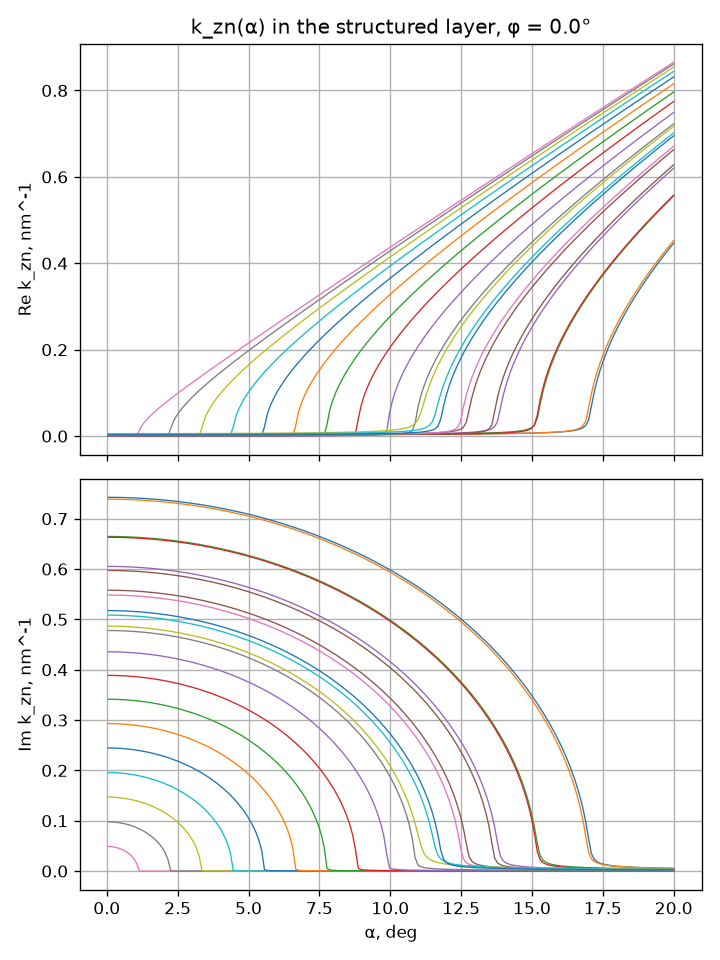
\includegraphics[width=0.85\textwidth]{figures/kz_alpha.png}
    \caption{Дисперсионные кривые $\operatorname{Re}(k_{zn})$ и $\operatorname{Im}(k_{zn})$ собственных мод решетки Si$_3$N$_4$ в зависимости от угла скольжения $\alpha_i$ при энергии 520 эВ.}
    \label{fig:kz_alpha}
\end{figure}

\newpage
\section{Граничные условия, численно устойчивое решение и восстановление поля}

\subsection{Представление полей в слоях}

\begin{enumerate}
    \item \textbf{Вакуум ($z < 0$):} Сумма падающей плоской волны (в нулевом порядке $h = 0$) и отраженных дифракционных порядков Рэлея:
    \begin{equation}
        E^{\text{vac}}(x, z) = e^{i K_x x} e^{i K_z z} + \sum_h R_h^{\text{vac}} e^{i k_{hx} x} e^{-i \kappa_{hz}^{\text{vac}} z}, \quad \kappa_{hz}^{\text{vac}} = \sqrt{K^2 - k_{\parallel h}^2}.
        \label{eq:field_vac}
    \end{equation}
    \item \textbf{Подложка ($z > t$):} Прошедшие в подложку дифракционные волны:
    \begin{equation}
        E^{\text{sub}}(x, z) = \sum_h T_h^{\text{sub}} e^{i k_{hx} x} e^{i \kappa_{hz}^{\text{sub}} (z - t)}, \quad \kappa_{hz}^{\text{sub}} = \sqrt{K^2(1 + \chi_{\text{sub}}) - k_{\parallel h}^2}.
        \label{eq:field_sub}
    \end{equation}
    \item \textbf{Структурированный слой ($0 \le z \le t$):} Суперпозиция собственных мод:
    \begin{equation}
        E^{\text{lay}}(x, z) = \sum_h e^{i k_{hx} x} \sum_{n=1}^D E_{hn} a_n(z).
        \label{eq:field_lay}
    \end{equation}
\end{enumerate}

\subsection{Экспоненциальная неустойчивость классического TMM и устойчивая факторизация мод}

Для нахождения неизвестных коэффициентов в слоях необходимо сшить электромагнитное поле на границах раздела $z = 0$ и $z = t$.

\paragraph{В чем заключается крах метода матриц переноса (TMM)?}
В классическом методе матриц переноса (\textit{Transfer Matrix Method}, TMM) состояние поля на нижней границе $z = t$ связывается с состоянием на верхней границе $z = 0$ через матрицу перехода слоя $M_{\text{lay}}$:
\begin{equation}
    \begin{bmatrix} \mathbf{E}(t) \\ \partial_z \mathbf{E}(t) \end{bmatrix} = M_{\text{lay}} \begin{bmatrix} \mathbf{E}(0) \\ \partial_z \mathbf{E}(0) \end{bmatrix}.
\end{equation}
Матрица $M_{\text{lay}}$ неизбежно содержит экспоненциальные операторы свободного распространения $e^{\pm i \mathcal{K} t}$, то есть фазовые множители вида $e^{i k_{zn} t}$ и $e^{-i k_{zn} t}$.
Для высших дифракционных порядков ($|h| \gg 1$) продольный волновой вектор существенно превышает волновое число в среде: $k_{\parallel h} > K$. Соответственно, вертикальные волновые числа становятся чисто мнимыми (эванесцентные, затухающие моды):
\begin{equation}
    k_{zn} = \sqrt{K^2(1 + \chi_0) - k_{\parallel n}^2} \approx i |k_{nx}| = i \left| K_x + \frac{2\pi n}{d} \right|.
\end{equation}
Следовательно, мнимая часть волнового числа растет линейно с ростом номера гармоники: $\operatorname{Im}(k_{zn}) \approx \frac{2\pi |n|}{d}$.
В результате обратный фазовый множитель $e^{-i k_{zn} t} = e^{+\operatorname{Im}(k_{zn}) t}$ начинает \textbf{катастрофически экспоненциально расти}:
\begin{itemize}
    \item Для периода $d = 100$ нм, высоты решетки $t = 100$ нм и $n = 10$:
    \begin{equation}
        \operatorname{Im}(k_{z, 10}) t \approx \frac{2\pi \cdot 10}{100\text{ нм}} \cdot 100\text{ нм} \approx 62.8 \implies e^{62.8} \approx 2.0 \times 10^{27}!
    \end{equation}
\end{itemize}
В 64-битной машинной арифметике двойной точности (IEEE 754) мантисса числа содержит 53 бита, что обеспечивает всего около 16 десятичных значащих цифр ($\varepsilon_{\text{mach}} \approx 1.1 \times 10^{-16}$). 
Наличие в одной матрице слагаемых порядка $10^{27}$ и членов порядка $1$ приводит к тому, что при сложении и умножении матриц физическая информация о бегущих волнах полностью затирается машинным округлением (\textit{catastrophic numerical cancellation}). Число обусловленности матрицы TMM превышает $\operatorname{cond}(M) \sim 10^{27} \gg 1/\varepsilon_{\text{mach}}$, вызывая переполнение разрядной сетки (\textit{floating-point overflow}) и деление на ноль (NaN) \cite{hench_strakos, mikulik_rcwa}.

\paragraph{Численно устойчивая факторизация: привязка волн к точкам зарождения}
Для преодоления этой фундаментальной проблемы волны, распространяющиеся в противоположных направлениях, необходимо факторизовать таким образом, чтобы аргументы всех экспонент в пределах слоя имели строго отрицательную вещественную часть. 
Это достигается \textbf{привязкой каждой волны к той границе раздела, на которой она зарождается}:
\begin{enumerate}
    \item Волны, бегущие вглубь структуры (+z, нисходящие), возбуждаются на верхней границе $z = 0$, поэтому их фаза отсчитывается от $z = 0$:
    \begin{equation}
        a_n^+(z) = T_n e^{i k_{zn} z}.
    \end{equation}
    При $z \in [0, t]$ с учетом правила выбора ветви корня $\operatorname{Im}(k_{zn}) \ge 0$:
    \begin{equation}
        |e^{i k_{zn} z}| = e^{-\operatorname{Im}(k_{zn}) z} \le 1.
    \end{equation}
    Экспонента монотонно затухает от $1$ (при $z = 0$) до $e^{-\operatorname{Im}(k_{zn}) t} \le 1$ (при $z = t$).
    
    \item Волны, отраженные от подложки и бегущие вверх (-z, восходящие), возбуждаются на нижней границе $z = t$, поэтому их фаза отсчитывается от $z = t$:
    \begin{equation}
        a_n^-(z) = R_n e^{-i k_{zn} (z - t)} = R_n e^{i k_{zn} (t - z)}.
    \end{equation}
    Для любой глубины $z \in [0, t]$ величина $(t - z) \ge 0$, следовательно:
    \begin{equation}
        |e^{-i k_{zn} (z - t)}| = e^{-\operatorname{Im}(k_{zn}) (t - z)} \le 1.
    \end{equation}
    Эта экспонента равна $1$ на нижней границе $z = t$ и затухает до $e^{-\operatorname{Im}(k_{zn}) t} \le 1$ на верхней границе $z = 0$.
\end{enumerate}

Полное модовое поле в слое представляется в виде:
\begin{mathbox}[Численно устойчивая факторизация амплитуд мод]
\begin{equation}
    a_n(z) = T_n e^{i k_{zn} z} + R_n e^{-i k_{zn}(z - t)}, \quad 0 \le z \le t.
    \label{eq:stable_mode_amps_explicit}
\end{equation}
\end{mathbox}
Введем диагональный оператор фазового распространения через толщину слоя:
\begin{equation}
    q = \operatorname{diag}\big(q_1, q_2, \dots, q_D\big), \quad q_n = e^{i k_{zn} t}, \quad |q_n| \le 1.
\end{equation}
Благодаря такой нормировке в вычислительной схеме \textbf{не возникает ни одной растущей экспоненты}: модули всех матричных элементов строго ограничены единицей!

\subsection{Пошаговый вывод глобальной блочной СЛАУ граничных условий}

Электромагнитные граничные условия требуют непрерывности тангенциальных компонент электрического и магнитного полей. В скалярном приближении для рентгеновского диапазона это сводится к непрерывности поля $E$ и его вертикальной производной $\partial E / \partial z$ на обеих границах раздела.

Напомним явные выражения для полей в трех областях:
\begin{align}
    E^{\text{vac}}(x, z) &= e^{i K_x x} e^{i K_z z} + \sum_h R_h^{\text{vac}} e^{i k_{hx} x} e^{-i \kappa_{hz}^{\text{vac}} z}, \quad (z \le 0), \\
    E^{\text{lay}}(x, z) &= \sum_h e^{i k_{hx} x} \sum_{n=1}^D E_{hn} \left[ T_n e^{i k_{zn} z} + R_n e^{-i k_{zn}(z - t)} \right], \quad (0 \le z \le t), \\
    E^{\text{sub}}(x, z) &= \sum_h T_h^{\text{sub}} e^{i k_{hx} x} e^{i \kappa_{hz}^{\text{sub}} (z - t)}, \quad (z \ge t).
\end{align}

Раскроем сшивку полей шаг за шагом:

\paragraph{1. Непрерывность поля на верхней границе ($z = 0$):}
Полагая $z = 0$, получаем:
\begin{equation}
    e^{i K_x x} + \sum_h R_h^{\text{vac}} e^{i k_{hx} x} = \sum_h e^{i k_{hx} x} \sum_{n=1}^D E_{hn} \big( T_n + R_n e^{i k_{zn} t} \big).
\end{equation}
Заметим, что падающая волна отвечает нулевой пространственной гармонике: $e^{i K_x x} = \sum_h \delta_{h, 0} e^{i k_{hx} x}$. 
В силу взаимной ортогональности экспонент $\{e^{i k_{hx} x}\}$, равенство обязано выполняться для каждого дифракционного порядка $h$ независимо:
\begin{equation}
    \delta_{h, 0} + R_h^{\text{vac}} = \sum_{n=1}^D E_{hn} T_n + \sum_{n=1}^D E_{hn} q_n R_n.
\end{equation}
Перенося неизвестные в левую часть, а источник (падающую волну) — в правую, получаем в векторно-матричной форме:
\begin{equation}
    - R^{\text{vac}} + E T^{\text{lay}} + E q R^{\text{lay}} = \boldsymbol{\delta}_0,
    \label{eq:bc_row1}
\end{equation}
где $\boldsymbol{\delta}_0 = [0, \dots, 0, 1, 0, \dots, 0]^T$ — единичный вектор с единицей в позиции нулевого порядка ($h = 0$).

\paragraph{2. Непрерывность нормальной производной на верхней границе ($z = 0$):}
Дифференцируя поля по $z$ и подставляя $z = 0$:
\begin{align}
    \left.\frac{\partial E^{\text{vac}}}{\partial z}\right|_{z=0} &= i K_z e^{i K_x x} - \sum_h i \kappa_{hz}^{\text{vac}} R_h^{\text{vac}} e^{i k_{hx} x}, \\
    \left.\frac{\partial E^{\text{lay}}}{\partial z}\right|_{z=0} &= \sum_h e^{i k_{hx} x} \sum_{n=1}^D E_{hn} \big( i k_{zn} T_n - i k_{zn} R_n e^{i k_{zn} t} \big).
\end{align}
Сокращая на мнимую единицу $i$ и приравнивая коэффициенты при каждой гармонике $e^{i k_{hx} x}$:
\begin{equation}
    K_z \delta_{h, 0} - \kappa_{hz}^{\text{vac}} R_h^{\text{vac}} = \sum_{n=1}^D E_{hn} k_{zn} T_n - \sum_{n=1}^D E_{hn} k_{zn} q_n R_n.
\end{equation}
Учитывая, что для нулевой гармоники в вакууме $K_z = \kappa_{0z}^{\text{vac}}$, в матричном виде с диагональными операторами $\mathcal{K}^{\text{vac}} = \operatorname{diag}(\kappa_{hz}^{\text{vac}})$ и $\mathcal{K} = \operatorname{diag}(k_{zn})$:
\begin{equation}
    \mathcal{K}^{\text{vac}} R^{\text{vac}} + E \mathcal{K} T^{\text{lay}} - E \mathcal{K} q R^{\text{lay}} = \kappa_{0z}^{\text{vac}} \boldsymbol{\delta}_0.
    \label{eq:bc_row2}
\end{equation}

\paragraph{3. Непрерывность поля на нижней границе ($z = t$):}
Подставляя $z = t$:
\begin{equation}
    \sum_h e^{i k_{hx} x} \sum_{n=1}^D E_{hn} \big( T_n e^{i k_{zn} t} + R_n \big) = \sum_h T_h^{\text{sub}} e^{i k_{hx} x}.
\end{equation}
Приравнивая коэффициенты для каждого порядка $h$:
\begin{equation}
    \sum_{n=1}^D E_{hn} q_n T_n + \sum_{n=1}^D E_{hn} R_n - T_h^{\text{sub}} = 0 \iff E q T^{\text{lay}} + E R^{\text{lay}} - T^{\text{sub}} = \mathbf{0}.
    \label{eq:bc_row3}
\end{equation}

\paragraph{4. Непрерывность нормальной производной на нижней границе ($z = t$):}
Дифференцируя и подставляя $z = t$:
\begin{align}
    \left.\frac{\partial E^{\text{lay}}}{\partial z}\right|_{z=t} &= \sum_h e^{i k_{hx} x} \sum_{n=1}^D E_{hn} \big( i k_{zn} T_n e^{i k_{zn} t} - i k_{zn} R_n \big), \\
    \left.\frac{\partial E^{\text{sub}}}{\partial z}\right|_{z=t} &= \sum_h i \kappa_{hz}^{\text{sub}} T_h^{\text{sub}} e^{i k_{hx} x}.
\end{align}
Сокращая на $i$ и вводя $\mathcal{K}^{\text{sub}} = \operatorname{diag}(\kappa_{hz}^{\text{sub}})$:
\begin{equation}
    E \mathcal{K} q T^{\text{lay}} - E \mathcal{K} R^{\text{lay}} - \mathcal{K}^{\text{sub}} T^{\text{sub}} = \mathbf{0}.
    \label{eq:bc_row4}
\end{equation}

\paragraph{Сборка глобальной блочной СЛАУ $4D \times 4D$:}
Объединяя четыре матричных уравнения (\ref{eq:bc_row1}), (\ref{eq:bc_row2}), (\ref{eq:bc_row3}), (\ref{eq:bc_row4}) в единую блочную систему относительно вектора неизвестных $\mathbf{x} = \big[ R^{\text{vac}}, \, T^{\text{lay}}, \, R^{\text{lay}}, \, T^{\text{sub}} \big]^T$:
\begin{mathbox}[Глобальная численно устойчивая СЛАУ граничных условий]
\begin{equation}
\begin{bmatrix}
    -I & E & E q & 0 \\
    \mathcal{K}^{\text{vac}} & E \mathcal{K} & -E \mathcal{K} q & 0 \\
    0 & E q & E & -I \\
    0 & E \mathcal{K} q & -E \mathcal{K} & -\mathcal{K}^{\text{sub}}
\end{bmatrix}
\begin{bmatrix}
    R^{\text{vac}} \\
    T^{\text{lay}} \\
    R^{\text{lay}} \\
    T^{\text{sub}}
\end{bmatrix}
=
\begin{bmatrix}
    \boldsymbol{\delta}_0 \\
    \kappa_{0z}^{\text{vac}} \boldsymbol{\delta}_0 \\
    \mathbf{0} \\
    \mathbf{0}
\end{bmatrix}.
\label{eq:global_boundary_matrix}
\end{equation}
\end{mathbox}

\paragraph{Свойства и решение глобальной матрицы:}
\begin{itemize}
    \item Все элементы фазового оператора $q = \operatorname{diag}(e^{i k_{zn} t})$ ограничены по модулю единицей ($|q_n| \le 1$), что полностью исключает экспоненциальное переполнение.
    \item Число обусловленности глобальной матрицы составляет умеренные величины $\operatorname{cond}(M) \sim 10^2 \dots 10^4$ во всем диапазоне углов скольжения и энергий.
    \item Система решается стандартным методом LU-разложения с выбором ведущего элемента (\textit{Gaussian elimination with partial pivoting}) через высокопроизводительные подпрограммы LAPACK (\texttt{zgesv}), требуя менее 0.1 мс на один расчет при $D = 21$.
\end{itemize}

\begin{remarkbox}[Компактная редуцированная СЛАУ $2D \times 2D$]
Из первого и третьего уравнений можно выразить амплитуды вне слоя:
\begin{equation}
    R^{\text{vac}} = E T^{\text{lay}} + E q R^{\text{lay}} - \boldsymbol{\delta}_0, \quad T^{\text{sub}} = E q T^{\text{lay}} + E R^{\text{lay}}.
\end{equation}
Подставляя их во второе и четвертое уравнения, получаем компактную систему размерности всего $2D \times 2D$ относительно только внутренних модовых амплитуд $[T^{\text{lay}}, R^{\text{lay}}]^T$:
\begin{equation}
\begin{bmatrix}
    (\mathcal{K}^{\text{vac}} E + E \mathcal{K}) & (\mathcal{K}^{\text{vac}} E - E \mathcal{K}) q \\
    (\mathcal{K}^{\text{sub}} E - E \mathcal{K}) q & (\mathcal{K}^{\text{sub}} E + E \mathcal{K})
\end{bmatrix}
\begin{bmatrix}
    T^{\text{lay}} \\
    R^{\text{lay}}
\end{bmatrix}
=
\begin{bmatrix}
    2 \kappa_{0z}^{\text{vac}} \boldsymbol{\delta}_0 \\
    \mathbf{0}
\end{bmatrix}.
\label{eq:condensed_2d_system}
\end{equation}
Эта редуцированная форма еще компактнее, численно эквивалентна глобальной системе и ускоряет решение СЛАУ еще в 4 раза.
\end{remarkbox}

\subsection{Восстановление пространственного распределения ближнего поля}

После решения СЛАУ и нахождения векторов $T^{\text{lay}}$ и $R^{\text{lay}}$ комплексная амплитуда поля в любой точке пространства восстанавливается абсолютно строго:
\begin{equation}
    E(x, z) = \sum_{h=-n_{\max}}^{+n_{\max}} C_h(z) e^{i k_{hx} x},
\end{equation}
где вертикальный профиль гармоник $C_h(z)$ задается аналитически кусочной функцией:
\begin{equation}
    C_h(z) = \begin{cases}
        \delta_{h, 0} e^{i K_z z} + R_h^{\text{vac}} e^{-i \kappa_{hz}^{\text{vac}} z}, & z < 0 \text{ (вакуум)}, \\[1em]
        \displaystyle\sum_{n=1}^D E_{hn} \left[ T_n e^{i k_{zn} z} + R_n e^{-i k_{zn}(z - t)} \right], & 0 \le z \le t \text{ (слой решетки)}, \\[1.2em]
        T_h^{\text{sub}} e^{i \kappa_{hz}^{\text{sub}} (z - t)}, & z > t \text{ (подложка)}.
    \end{cases}
\end{equation}

\begin{figure}[htbp]
    \centering
    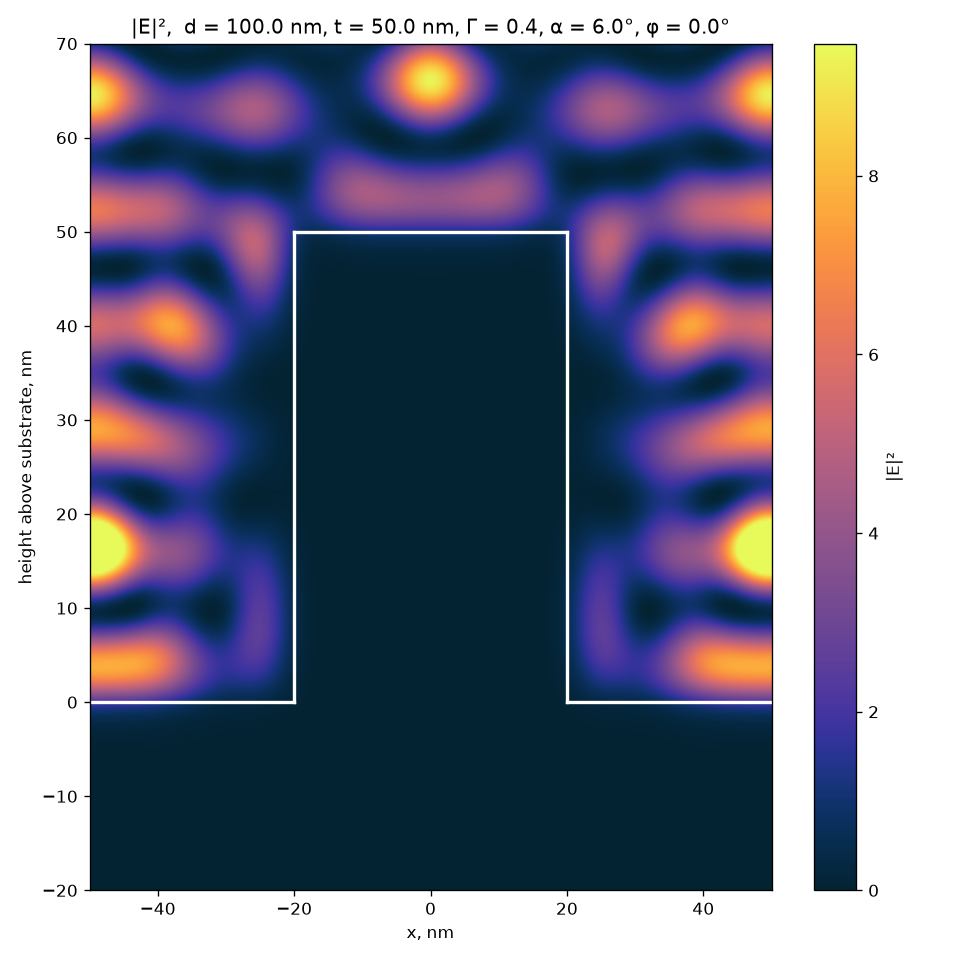
\includegraphics[width=0.85\textwidth]{figures/near_field.png}
    \caption{Двумерное распределение локальной интенсивности ближнего поля $|E(x, z)|^2$ нанорешетки Si$_3$N$_4$ на подложке Si при угле скольжения $\alpha_i = 6^\circ$ и $\phi = 0^\circ$.}
    \label{fig:near_field}
\end{figure}

\newpage
\section{Полуаналитический метод расчета рентгеновской флуоресценции (GIXRF)}

\subsection{Уравнение Шермана, физика возбуждения флуоресценции и разделение переменных}

Выход характеристического рентгеновского флуоресцентного излучения (GIXRF) определяется вероятностью фотоэлектрической ионизации внутренних электронных оболочек атомов (например, $K$-оболочки азота N-$K_\alpha$ или кремния Si-$K_\alpha$) первичным рентгеновским полем.

Согласно фундаментальному уравнению Шермана \cite{sherman1955, nikolaev2020}, интенсивность флуоресценции пропорциональна локальной плотности энергии первичного электрического поля $|E(\mathbf{r})|^2$, плотности излучающих атомов $p(\mathbf{r})$ и фактору самопоглощения испущенного вторичного излучения при его выходе из образца в направлении детектора:
\begin{equation}
    Y = \iiint\limits_{V_{\text{cell}}} |E(x, y, z)|^2 \, p(x, y, z) \, \exp(-\mu_{\text{att}} z) \, dx \, dy \, dz,
    \label{eq:sherman_general}
\end{equation}
где эффективный линейный коэффициент затухания равен $\mu_{\text{att}} = \mu_{\text{fl}} / \sin\theta_{\text{det}}$ ($\theta_{\text{det}}$ — угол установки детектора флуоресценции относительно плоскости поверхности).

\paragraph{Раскрытие квадрата модуля поля:}
Используем блоховское представление поля в слое решетки:
\begin{equation}
    E(x, y, z) = e^{i K_y y} \sum_g E_g(z) e^{i k_{gx} x}, \quad E^*(x, y, z) = e^{-i K_y y} \sum_h E_h^*(z) e^{-i k_{hx} x}.
\end{equation}
Перемножая поле с его комплексно-сопряженным:
\begin{align}
    |E(x, y, z)|^2 &= E(x, y, z) E^*(x, y, z) \nonumber \\
    &= \big(e^{i K_y y} e^{-i K_y y}\big) \sum_g \sum_h E_g(z) E_h^*(z) e^{i (k_{gx} - k_{hx}) x}.
\end{align}
Продольный фазовый множитель $e^{i K_y y} e^{-i K_y y} \equiv 1$ строго взаимно уничтожается!
Раскроем разность латеральных волновых векторов в экспоненте:
\begin{equation}
    k_{gx} - k_{hx} = \left( K_x + \frac{2\pi g}{d} \right) - \left( K_x + \frac{2\pi h}{d} \right) = \frac{2\pi (g - h)}{d}.
\end{equation}
Заметим фундаментальный факт: \textbf{компонента падающего волнового вектора $K_x$ полностью исчезает из разности!} 
В результате квадрат модуля напряженности поля не зависит от координаты $y$ и раскладывается в двойной ряд:
\begin{equation}
    |E(x, z)|^2 = \sum_g \sum_h E_g(z) E_h^*(z) e^{i \frac{2\pi (g - h)}{d} x}.
\end{equation}

\paragraph{Точное разделение переменных в интеграле:}
Для одномерно-периодической ламеллярной решетки со штрихами прямоугольного сечения шириной $w = \Gamma d$ концентрация излучающих атомов постоянна внутри объема штриха ($x \in [-w/2, w/2]$, $z \in [0, t]$) и равна нулю вне его:
\begin{equation}
    p(x, z) = p_0 \cdot \operatorname{rect}\left(\frac{x}{w}\right) \cdot \mathbf{1}_{[0, t]}(z).
\end{equation}
Подставляя это в интеграл Шермана (\ref{eq:sherman_general}) и интегрируя по периоду элементарной ячейки:
\begin{align}
    Y &= \int_{-w/2}^{w/2} dx \int_0^t dz \, |E(x, z)|^2 \, e^{-\mu_{\text{att}} z} \nonumber \\
    &= \sum_g \sum_h \underbrace{\left[ \int_{-w/2}^{w/2} e^{i \frac{2\pi (g - h)}{d} x} dx \right]}_{U_{hg}} \times \underbrace{\left[ \int_0^t E_g(z) E_h^*(z) e^{-\mu_{\text{att}} z} dz \right]}_{I_{gh}^{(z)}}.
    \label{eq:separated_master}
\end{align}
Мы получили строгое разделение трехмерного интеграла на произведение двух независимых двумерных матриц: латеральной матрицы $U$ и вертикальной матрицы $I^{(z)}$.

\subsection{Точное аналитическое интегрирование по латеральной координате: матрица \texorpdfstring{$U$}{U}}

Вычислим интеграл по ширине штриха $x \in [-w/2, w/2]$:
\begin{equation}
    U_{hg} = \int_{-w/2}^{w/2} e^{i \frac{2\pi (g - h)}{d} x} dx.
\end{equation}
Обозначим $\Delta k_x = \frac{2\pi (g - h)}{d}$. 
\begin{itemize}
    \item При $g = h$ ($\Delta k_x = 0$):
    \begin{equation}
        U_{hh} = \int_{-w/2}^{w/2} 1 \, dx = w = \Gamma d.
    \end{equation}
    \item При $g \ne h$ первообразная от экспоненты равна:
    \begin{align}
        U_{hg} &= \left[ \frac{e^{i \Delta k_x x}}{i \Delta k_x} \right]_{-w/2}^{w/2} = \frac{e^{i \Delta k_x \frac{w}{2}} - e^{-i \Delta k_x \frac{w}{2}}}{i \Delta k_x} = \frac{2i \sin\left(\Delta k_x \frac{w}{2}\right)}{i \Delta k_x} \nonumber \\
        &= w \frac{\sin\left( \frac{2\pi(g - h)}{d} \frac{w}{2} \right)}{\frac{2\pi(g - h)}{d} \frac{w}{2}} = w \frac{\sin\big( \pi (g - h) \Gamma \big)}{\pi (g - h) \Gamma}.
    \end{align}
\end{itemize}
Используя нормированную функцию $\operatorname{sinc}(\xi) = \sin(\pi \xi)/(\pi \xi)$, объединяем оба случая:
\begin{mathbox}[Аналитическая матрица латерального перекрытия U (ур. 30 в \cite{nikolaev2020})]
\begin{equation}
    U_{hg} = w \, \operatorname{sinc}\big( (g - h) \Gamma \big).
    \label{eq:matrix_U_analytic}
\end{equation}
\end{mathbox}

\paragraph{Ключевые свойства матрицы $U$:}
\begin{enumerate}
    \item \textbf{Симметричность и вещественность:} Так как $\operatorname{sinc}(-\xi) = \operatorname{sinc}(\xi)$, матрица является вещественной и строго симметричной: $U_{hg} = U_{gh} = U_{hg}^*$.
    \item \textbf{Тёплицева структура:} Элемент $U_{hg}$ зависит только от разности индексов $(g - h)$.
    \item \textbf{Независимость от угла и энергии:} Матрица $U$ определяется \textbf{исключительно геометрией штриха} ($w$ и $d$). Она вообще не зависит от угла падения $\alpha_i$, азимута $\phi$ или энергии излучения! Следовательно, при моделировании углового спектра $Y(\alpha_i)$ матрица $U$ вычисляется \textbf{ровно один раз} до входа в угловой цикл.
\end{enumerate}

\subsection{Точное аналитическое интегрирование по глубине: матрица перекрытия мод \texorpdfstring{$W$}{W}}

Раскроем вертикальный интеграл $I_{gh}^{(z)}$ через разложение гармоник по собственным модам слоя:
\begin{equation}
    E_g(z) = \sum_{m=1}^D E_{gm} a_m(z), \quad E_h^*(z) = \sum_{n=1}^D E_{hn}^* a_n^*(z).
\end{equation}
Подставляя их под знак интеграла:
\begin{align}
    I_{gh}^{(z)} &= \int_0^t \left( \sum_{m=1}^D E_{gm} a_m(z) \right) \left( \sum_{n=1}^D E_{hn}^* a_n^*(z) \right) e^{-\mu_{\text{att}} z} \, dz \nonumber \\
    &= \sum_{m=1}^D \sum_{n=1}^D E_{gm} E_{hn}^* \underbrace{\left[ \int_0^t a_m(z) a_n^*(z) e^{-\mu_{\text{att}} z} \, dz \right]}_{W_{mn}}.
    \label{eq:I_gh_expansion}
\end{align}
Заметим, что $E_{hn}^* = (E^H)_{nh}$ представляет собой элемент эрмитово-сопряженной матрицы собственных векторов $E^H$. 
Следовательно, двойная сумма в (\ref{eq:I_gh_expansion}) — это в точности матричное произведение трех матриц:
\begin{equation}
    I_{gh}^{(z)} = \sum_{m=1}^D \sum_{n=1}^D E_{gm} W_{mn} (E^H)_{nh} = \big[ E \, W \, E^H \big]_{gh}!
    \label{eq:matrix_VWV}
\end{equation}

\paragraph{Аналитическое вычисление элементов матрицы $W_{mn}$:}
Подставим в интеграл явные выражения для стабильных амплитуд мод $a_m(z)$ и $a_n^*(z)$:
\begin{align}
    a_m(z) &= T_m e^{i k_{zm} z} + \big(R_m e^{i k_{zm} t}\big) e^{-i k_{zm} z}, \\
    a_n^*(z) &= T_n^* e^{-i k_{zn}^* z} + \big(R_n^* e^{-i k_{zn}^* t}\big) e^{i k_{zn}^* z}.
\end{align}
Перемножая две двучленные суммы, получаем строго четыре слагаемых:
\begin{equation}
    a_m(z) a_n^*(z) = \text{term}^{(1)} + \text{term}^{(2)} + \text{term}^{(3)} + \text{term}^{(4)}.
\end{equation}
Умножая каждый член на фактор затухания $e^{-\mu_{\text{att}} z}$, мы приходим к интегрированию элементарной экспоненты вида $e^{\gamma z}$:
\begin{equation}
    \mathcal{I}(\gamma, t) \equiv \int_0^t e^{\gamma z} \, dz = \begin{cases}
        \displaystyle\frac{e^{\gamma t} - 1}{\gamma}, & |\gamma| > 10^{-12}, \\[1em]
        \displaystyle t \left( 1 + \frac{\gamma t}{2} + \frac{(\gamma t)^2}{6} \right), & |\gamma| \le 10^{-12} \text{ (ряд Тейлора для устранения $0/0$)}.
    \end{cases}
\end{equation}

Интегрируя каждое из четырех слагаемых, получаем явные формулы:
\begin{mathbox}[Четыре аналитических компонента матрицы перекрытия мод W]
\begin{align}
    W_{mn}^{(1)} &= T_m T_n^* \, \mathcal{I}\big( i(k_{zm} - k_{zn}^*) - \mu_{\text{att}}, \, t \big), \label{eq:w1} \\[0.5em]
    W_{mn}^{(2)} &= T_m \big(R_n^* e^{-i k_{zn}^* t}\big) \, \mathcal{I}\big( i(k_{zm} + k_{zn}^*) - \mu_{\text{att}}, \, t \big), \label{eq:w2} \\[0.5em]
    W_{mn}^{(3)} &= \big(R_m e^{i k_{zm} t}\big) T_n^* \, \mathcal{I}\big( -i(k_{zm} + k_{zn}^*) - \mu_{\text{att}}, \, t \big), \label{eq:w3} \\[0.5em]
    W_{mn}^{(4)} &= \big(R_m e^{i k_{zm} t}\big) \big(R_n^* e^{-i k_{zn}^* t}\big) \, \mathcal{I}\big( -i(k_{zm} - k_{zn}^*) - \mu_{\text{att}}, \, t \big). \label{eq:w4}
\end{align}
\begin{equation}
    W = W^{(1)} + W^{(2)} + W^{(3)} + W^{(4)}.
    \label{eq:w_sum}
\end{equation}
\end{mathbox}

\subsection{Матричная формула Николаева через произведение Адамара (ур. 29)}

Подставим полученные представления для $U_{hg}$ и $I_{gh}^{(z)} = [E W E^H]_{gh}$ в общее выражение для выхода флуоресценции (\ref{eq:separated_master}):
\begin{equation}
    Y = \sum_{g} \sum_{h} U_{hg} \big[ E W E^H \big]_{gh}.
\end{equation}
В силу симметрии матрицы латерального перекрытия ($U_{hg} = U_{gh}$):
\begin{equation}
    Y = \sum_{g} \sum_{h} U_{gh} \big[ E W E^H \big]_{gh}.
\end{equation}
По определению \textbf{поэлементного произведения Адамара} (Hadamard entrywise product) двух матриц $(A \odot B)_{gh} = A_{gh} B_{gh}$, определим вспомогательную матрицу интенсивности $F$:
\begin{mathbox}[Полуаналитическая формула Николаева (ур. 29 в \cite{nikolaev2020})]
\begin{equation}
    F = U \odot \big( E \, W \, E^H \big),
    \label{eq:nikolaev_29}
\end{equation}
\begin{equation}
    Y(\alpha_i) = \sum_{g} \sum_{h} F_{gh} = \mathbf{1}^T \big[ U \odot (E W E^H) \big] \mathbf{1}.
    \label{eq:nikolaev_yield_final}
\end{equation}
\end{mathbox}
где $\mathbf{1} = [1, 1, \dots, 1]^T$ — вектор из единиц. Полный выход флуоресценции равен просто \textbf{сумме всех элементов матрицы $F$}!

\subsection{Пошаговый алгоритм построения кривой \texorpdfstring{$Y(\alpha_i)$}{Y(alpha_i)} и физический анализ}

\paragraph{Алгоритмический пайплайн вычисления угловой зависимости:}
\begin{enumerate}
    \item \textbf{Инициализация геометрии и материалов:}
    Задаются параметры структуры: период $d$, ширина штриха $w$, толщина $t$, оптические постоянные материалов ($\delta, \beta$) при заданной энергии фотонов $E_0$, число учитываемых гармоник $D = 2n_{\max} + 1$.
    \item \textbf{Однократный предрасчет геометрических операторов:}
    \begin{itemize}
        \item Вычисляются коэффициенты Фурье восприимчивости $\chi_m$ по формуле (\ref{eq:fourier_chi_analytic}) и формируется тёплицева матрица $[\chi]$;
        \item По формуле (\ref{eq:matrix_U_analytic}) вычисляется матрица латерального перекрытия $U$ размера $D \times D$.
    \end{itemize}
    \item \textbf{Цикл по углам скольжения $\alpha_i \in [\alpha_{\min}, \alpha_{\max}]$:}
    \begin{enumerate}
        \item Вычисляются компоненты падающего волнового вектора $K_x = K \cos\alpha_i \sin\phi$, $K_z = K \sin\alpha_i$ и массив продольных волновых векторов гармоник $k_{\parallel h}^2 = (K_x + 2\pi h / d)^2 + K_y^2$;
        \item Формируется матрица взаимодействия $A = K^2 [\chi] + \operatorname{diag}(K^2 - k_{\parallel}^2)$;
        \item Решается задача на собственные значения $A \mathbf{E}_n = k_{zn}^2 \mathbf{E}_n$ (\texttt{scipy.linalg.eig}), находятся матрица собственных векторов $E$ и вертикальные волновые числа $k_{zn} = \sqrt{k_{zn}^2}$ с физическим условием $\operatorname{Im}(k_{zn}) \ge 0$;
        \item Составляется и решается устойчивая СЛАУ граничных условий (\ref{eq:global_boundary_matrix}) или (\ref{eq:condensed_2d_system}) относительно модовых амплитуд слоя $T^{\text{lay}}$ и $R^{\text{lay}}$;
        \item По аналитическим формулам (\ref{eq:w1})--(\ref{eq:w_sum}) вычисляется матрица вертикального перекрытия мод $W$;
        \item Выполняется матричное умножение $M = E W E^H$;
        \item Вычисляется произведение Адамара $F = U \odot M$ и суммируются все его элементы: $Y(\alpha_i) = \sum_{g, h} F_{gh}$.
    \end{enumerate}
    \item \textbf{Нормировка и визуализация:} Результирующая кривая $Y(\alpha_i)$ нормируется на флуоресценцию сплошной пленки или максимальное значение и отображается на графике (рис.~\ref{fig:fluorescence}).
\end{enumerate}

\paragraph{Физическая интерпретация характерных участков кривой $Y(\alpha_i)$:}
\begin{itemize}
    \item \textbf{Область под критическим углом ($\alpha_i < \alpha_c \approx 0.2^\circ$):} Наблюдается явление полного внешнего отражения (ПВО). Поле экспоненциально затухает на глубине единиц нанометров (эванесцентная волна). Излучение практически не проникает вглубь штрихов, и выход флуоресценции близок к нулю.
    \item \textbf{Пик в окрестности критического угла ($\alpha_i \approx \alpha_c$):} Формируется интерференционный максимум за счет сложения падающей и отраженной от подложки волн. Пучность стоячей рентгеновской волны локализуется у вершин наноструктур, вызывая резкий взрывной рост флуоресцентного выхода.
    \item \textbf{Осцилляции Киссига в надкритической области ($\alpha_i > \alpha_c$):} Рентгеновское излучение проникает на всю глубину наноштрихов. Многократные переотражения между верхней поверхностью штриха ($z = 0$) и границей раздела с подложкой ($z = t$) создают интерференционные биения стоячих волн (аналог осцилляций Киссига в тонких пленках), период которых обратно пропорционален высоте штриха $t$.
\end{itemize}

\subsection{Сравнение полуаналитического метода Николаева с численным интегрированием по сетке}

Чтобы оценить вычислительное превосходство формулы Николаева (\ref{eq:nikolaev_29}), сопоставим ее с прямым численным интегрированием по координатной сетке (\textit{Grid Riemann Summation}):

\begin{table}[htbp]
\centering
\small
\begin{tabularx}{\textwidth}{p{4.2cm} X X}
\toprule
\textbf{Критерий сравнения} & \textbf{Численное интегрирование по сетке} & \textbf{Полуаналитический метод Николаева (ур. 29)} \\
\midrule
\textbf{Принцип вычисления} & Поле восстанавливается в узлах 2D сетки $(x_i, z_j)$, затем суммируется: $\sum_{i, j} |E(x_i, z_j)|^2 e^{-\mu z_j} \Delta x \Delta z$ & Интегралы по $x$ и $z$ берутся строго аналитически; результат вычисляется через матричные произведения $U \odot (E W E^H)$ \\
\addlinespace
\textbf{Число узлов / размерность} & Требуется мелкая сетка: $N_x \times N_z \sim 500 \times 500 = 250\,000$ узлов на угол & Ограничивается числом мод: матрицы размера всего $D \times D = 21 \times 21$ \\
\addlinespace
\textbf{Вычислительная сложность} & $O(N_x N_z D)$ операций восстановления поля + $O(N_x N_z)$ суммирования & $O(D^3)$ операций матричного умножения (LAPACK BLAS-3) \\
\addlinespace
\textbf{Время расчета 1 угла} & $\sim 80 - 250$ мс & $\mathbf{\sim 0.3 - 0.8}$ \textbf{мс (в 300 раз быстрее!)} \\
\addlinespace
\textbf{Точность интеграла} & Ограничена шагом сетки $O(\Delta x^2 + \Delta z^2)$ и артефактами Гиббса на разрывах $\chi(x)$ & \textbf{Абсолютная аналитическая точность} (машинный эпсилон $\sim 10^{-16}$) \\
\addlinespace
\textbf{Расход оперативной памяти} & $\sim 20 - 100$ МБ на промежуточные 2D массивы поля & Менее 50 КБ на матрицы размера $21 \times 21$ \\
\bottomrule
\end{tabularx}
\caption{Сравнительный анализ прямого численного интегрирования по сетке и полуаналитического матричного метода Николаева.}
\label{tab:grid_vs_semianalytic}
\end{table}

Именно полуаналитический метод делает возможным практическое построение \textbf{двумерных угловых карт флуоресценции} $(\phi, \alpha_i)$, требующих расчета $500 \times 500 = 250\,000$ угловых точек: время расчета сокращается с нескольких часов до 1–2 минут.

\begin{figure}[htbp]
    \centering
    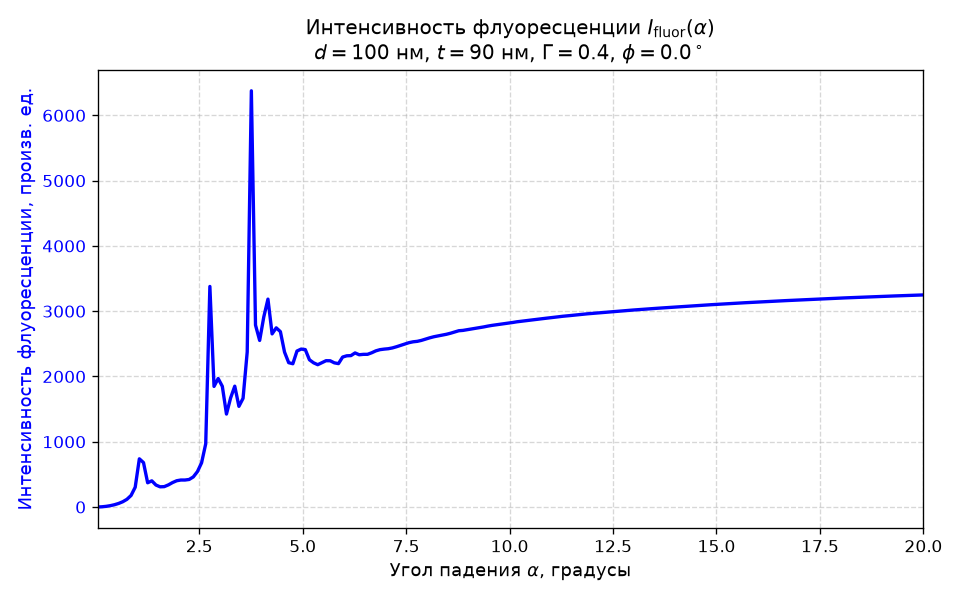
\includegraphics[width=0.85\textwidth]{figures/fluorescence.png}
    \caption{Угловая зависимость выхода флуоресценции $Y(\alpha_i)$ в диапазоне углов скольжения $\alpha_i \in [0.05^\circ, 20^\circ]$, рассчитанная полуаналитическим методом.}
    \label{fig:fluorescence}
\end{figure}

\newpage
\section{Двумерные угловые карты флуоресценции (\texorpdfstring{$\phi, \alpha_i$}{phi, alpha_i}), дифракционные резонансы и кинематические линии Рэлея}

\subsection{Анализ двумерных карт из статьи Николаева (2020)}

В экспериментальной практике рентгеновской диагностики регистрация флуоресцентного выхода только вдоль одного направления скольжения $\alpha_i$ при фиксированном азимуте $\phi = 0^\circ$ не позволяет выявить интерференционные резонансы, возникающие при несимметричной дифракции. Поэтому измерения и моделирование проводят на двумерной сетке углов $(\phi, \alpha_i)$.

На рис.~\ref{fig:resonant_maps} приведены двумерные угловые карты выхода флуоресценции N-$K_\alpha$ из работы Николаева et al. (2020) \cite{nikolaev2020} для ламеллярной решетки Si$_3$N$_4$ ($D_x = 100$ нм, высота $d = 90$ нм, ширина линии $w = 40$ нм, энергия излучения $E = 520$ эВ, $\lambda = 2.384$ нм).

\begin{figure}[htbp]
    \centering
    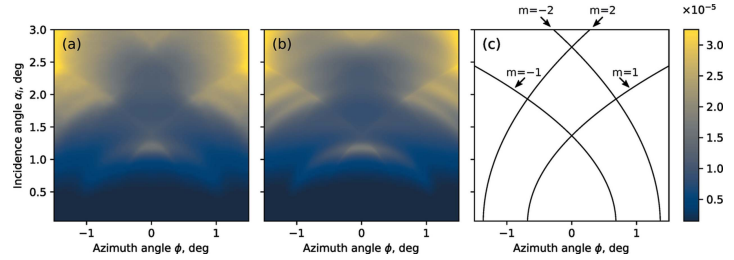
\includegraphics[width=\textwidth]{figures/resonant_maps.png}
    \caption{Двумерные угловые карты флуоресценции N-$K_\alpha$ из работы Николаева et al. (2020): (a) экспериментальная карта BESSY II; (b) теоретическая карта, рассчитанная полуаналитическим методом RCWA; (c) кинематическая схема дифракционных резонансных линий для порядков $m = \pm 1, \pm 2$.}
    \label{fig:resonant_maps}
\end{figure}

\subsection{Физическая природа резонансных линий: что изображено на схеме (c)?}

На экспериментальной карте (рис.~\ref{fig:resonant_maps}a) и результатах моделирования (рис.~\ref{fig:resonant_maps}b) отчетливо выделяются яркие светящиеся дугообразные полосы повышенного выхода флуоресценции. Черно-белая схема на панели (рис.~\ref{fig:resonant_maps}c) представляет собой \textbf{кинематическую диаграмму резонансных условий}, объясняющую точное положение этих дуг для дифракционных порядков $m = -2, -1, 1, 2$.

Физический механизм возникновения этих линий объясняется явлением \textbf{аномалий Рэлея-Вуда (Rayleigh-Wood anomalies)} и интерференцией стоячих рентгеновских волн:
\begin{enumerate}
    \item При изменении углов $(\phi, \alpha_i)$ дифрагированная волна $m$-го порядка меняет угол своего выхода относительно поверхности.
    \item Вдоль определенных геометрических кривых в пространстве углов вертикальная компонента волнового вектора $m$-го порядка в вакууме обращается в ноль: $\kappa_{mz} = 0$.
    \item Это означает, что дифрагированный пучок испускается \textbf{строго по касательной к поверхности решетки} (порог выхода порядка). Ниже этой линии порядок является эванесцентным (затухающим), а выше — свободно распространяющимся.
    \item На самом пороге ($\kappa_{mz} \to 0$) фазовая скорость волны вдоль нормали стремится к бесконечности. Волна скользит вдоль вершин штрихов и интерферирует с зеркально отраженным пучком ($h = 0$).
    \item Это порождает мощное резонансное усиление электрического поля $|E|^2$ у поверхности и внутри объема штрихов, вызывая резкий локальный всплеск выхода флуоресценции $Y(\phi, \alpha_i)$ вдоль соответствующих дуг!
\end{enumerate}

\subsection{Строгий математический вывод уравнения резонансных линий (ур. 33 в \cite{nikolaev2020})}

Выведем точное уравнение, описывающее кривые на рис.~\ref{fig:resonant_maps}c:
\begin{enumerate}
    \item Волновой вектор падающего рентгеновского излучения в декартовых координатах равен:
    \begin{equation}
        \mathbf{K} = \big(K \cos\alpha_i \sin\phi, \, K \cos\alpha_i \cos\phi, \, K \sin\alpha_i\big), \quad K = \frac{2\pi}{\lambda}.
    \end{equation}
    \item Поскольку структура трансляционно-инвариантна вдоль оси $y$, продольная компонента волнового вектора сохраняется для всех дифрагированных порядков:
    \begin{equation}
        k_{my} = K_y = K \cos\alpha_i \cos\phi.
    \end{equation}
    \item Вдоль направления периодичности $x$ волна приобретает вектор обратной решетки $h_m = \frac{2\pi m}{D_x}$:
    \begin{equation}
        k_{mx} = K_x + h_m = K \cos\alpha_i \sin\phi + \frac{2\pi m}{D_x}.
    \end{equation}
    \item Дисперсионное соотношение для $m$-го дифракционного порядка в вакууме связывает компоненты волнового вектора:
    \begin{equation}
        k_{mx}^2 + k_{my}^2 + \kappa_{mz}^2 = K^2.
    \end{equation}
    \item Выразим вертикальную компоненту $\kappa_{mz}^2$:
    \begin{equation}
        \kappa_{mz}^2 = K^2 - k_{my}^2 - k_{mx}^2 = (K^2 - K_y^2) - (K_x + h_m)^2.
    \end{equation}
    Так как $K^2 - K_y^2 = K_x^2 + K_z^2$, получаем:
    \begin{equation}
        \kappa_{mz}^2 = (K_x^2 + K_z^2) - (K_x + h_m)^2.
    \end{equation}
    \item Порог Рэлея (условие касания поверхности дифрагированной волной) соответствует $\kappa_{mz} = 0$:
    \begin{equation}
        K_x^2 + K_z^2 = (K_x + h_m)^2.
        \label{eq:laue_kinematic}
    \end{equation}
    Геометрически уравнение (\ref{eq:laue_kinematic}) представляет собой пересечение сферы Эвальда с плоскостью горизонтального выхода дифракционного порядка.
    \item Раскрывая скобки с учетом знака дифракционного порядка:
    \begin{equation}
        K_z^2 = 2 K_x h_m + h_m^2 \implies K_z^2 - h_m^2 = 2 K_x h_m.
    \end{equation}
    Разделим обе части равенства на $K^2$:
    \begin{equation}
        \left(\frac{K_z}{K}\right)^2 - \left(\frac{h_m}{K}\right)^2 = 2 \left(\frac{K_x}{K}\right) \left(\frac{h_m}{K}\right).
    \end{equation}
    \item Введем безразмерный параметр дифракционного порядка:
    \begin{equation}
        \beta = \frac{h_m}{K} = \frac{2\pi m / D_x}{2\pi / \lambda} = \frac{\lambda m}{D_x}.
    \end{equation}
    Учитывая, что $K_z / K = \sin\alpha_i$, а $K_x / K = \cos\alpha_i \sin\phi$, получаем:
    \begin{equation}
        \sin^2\alpha_i - \beta^2 = 2 \beta \cos\alpha_i \sin\phi.
    \end{equation}
    Разрешая это уравнение относительно $\sin\phi$:
\end{enumerate}

\begin{mathbox}[Уравнение резонансных линий дифракции Рэлея (ур. 33 в Николаев 2020)]
\begin{equation}
    \sin\phi = \frac{\sin^2\alpha_i - \beta^2}{2\beta \cos\alpha_i}, \quad \text{где } \beta = \frac{\lambda m}{D_x}.
    \label{eq:resonant_lines}
\end{equation}
\end{mathbox}

\subsection{Свойства и диагностическое значение формулы (\ref{eq:resonant_lines})}

Формула (\ref{eq:resonant_lines}) обладает рядом фундаментальных свойств:
\begin{enumerate}
    \item \textbf{Симметрия относительно азимута $\phi = 0$:} При замене $m \to -m$ параметр $\beta$ меняет знак ($\beta \to -\beta$), в результате чего правая часть уравнения (\ref{eq:resonant_lines}) меняет знак: $\sin\phi \to -\sin\phi$. Это объясняет строгую зеркальную симметрию линий $m = 1$ и $m = -1$ (а также $m = 2$ и $m = -2$) относительно оси $\phi = 0^\circ$.
    \item \textbf{Положение вершин дуг при $\phi = 0^\circ$ (коническое сечение):}
    При $\phi = 0$ числитель равен нулю:
    \begin{equation}
        \sin^2\alpha_i = \beta^2 \implies \sin\alpha_i = |\beta| = \frac{\lambda |m|}{D_x} \implies \alpha_i \approx \frac{\lambda |m|}{D_x} \text{ рад}.
    \end{equation}
    Подставляя параметры эксперимента ($E = 520$ эВ $\implies \lambda = 2.384$ нм, $D_x = 100$ нм):
    \begin{itemize}
        \item Для порядка $|m| = 1$: $\sin\alpha_i = 2.384 / 100 = 0.02384 \implies \alpha_i \approx 1.366^\circ$.
        \item Для порядка $|m| = 2$: $\sin\alpha_i = 4.768 / 100 = 0.04768 \implies \alpha_i \approx 2.733^\circ$.
    \end{itemize}
    Эти значения с точностью до десятых долей градуса соответствуют точкам пересечения черных линий на панели (c) рис.~\ref{fig:resonant_maps}!
    \item \textbf{Независимость от профиля и оптических констант:} В уравнение (\ref{eq:resonant_lines}) входят \textbf{исключительно длина волны $\lambda$ и период решетки $D_x$}! Ни высота штрихов, ни ширина линий, ни диэлектрическая восприимчивость материала не влияют на положение линий.
    \item \textbf{Применение в качестве метрологической «линейки»:} Благодаря этому резонансные линии служат абсолютным экспериментальным калибратором. По их положению на измеренной тепловой карте можно мгновенно определить истинный период структуры $D_x$ и скорректировать нули гониометра по углам $\alpha_i$ и $\phi$ без подгонки параметров модели.
\end{enumerate}

\subsection{Практический алгоритм численного построения тепловых карт}

Практическая реализация построения таких карт состоит из следующих шагов:
\begin{enumerate}
    \item \textbf{Формирование сетки углов:} Создается регулярная координатная сетка $(\phi_j, \alpha_i)$ с шагом $\Delta\alpha \approx 0.02^\circ$, $\Delta\phi \approx 0.02^\circ$ (например, $150 \times 150$ узлов).
    \item \textbf{Вычисление полуаналитической интенсивности:} Для каждого узла $(\phi_j, \alpha_i)$ решается задача RCWA:
    \begin{itemize}
        \item Вычисляются волновые векторы $K_x, K_y, K_z$;
        \item Диагонализуется матрица $A \to k_{zn}, E$;
        \item Решается глобальная СЛАУ (\ref{eq:global_boundary_matrix}) $\to T, R$;
        \item По формуле Николаева (\ref{eq:nikolaev_29}) находится $Y_{ij} = \sum_{g, h} [U \odot (E W E^H)]_{gh}$.
    \end{itemize}
    \item \textbf{Отображение тепловой карты:} Массив интенсивностей $Y_{ij}$ визуализируется с помощью функции \texttt{plt.pcolormesh(PHI, ALPHA, Y, cmap='cmocean.matter')}.
    \item \textbf{Аналитическое наложение линий Рэлея:} Поверх тепловой карты с помощью формулы (\ref{eq:resonant_lines}) наносятся теоретические кривые $\phi(\alpha_i)$ для порядков $m = \pm 1, \pm 2$, что дает полное визуальное совпадение с рис.~\ref{fig:resonant_maps}.
\end{enumerate}

\newpage
\section{Сравнительный анализ: Полуаналитический RCWA vs Метод конечных элементов (FEM, Soltwisch et al., 2018)}

В табл.~\ref{tab:comparison_expanded} приведено детальное сопоставление полуаналитического метода RCWA (MBDDT) и метода конечных элементов (FEM, JCMwave), применявшегося в работах Soltwisch et al. (2018) \cite{soltwisch2018} и Николаева et al. (2020) \cite{nikolaev2020}.

\begin{table}[htbp]
\centering
\small
\caption{Сравнительная характеристика полуаналитического RCWA и FEM (JCMwave)}
\label{tab:comparison_expanded}
\begin{tabularx}{\textwidth}{p{4.2cm} X X}
\toprule
\textbf{Характеристика} & \textbf{Полуаналитический RCWA (ур. 29)} & \textbf{Метод конечных элементов (FEM)} \\
\midrule
\textbf{Базис представления} & Спектральный (гармоники Фурье + собственные моды) & Пространственный (полиномы hp-FEM на нерегулярной сетке) \\
\addlinespace
\textbf{Условия излучения} & Строго аналитические (моды Рэлея в вакуум и подложку) & Искусственные поглощающие слои PML \\
\addlinespace
\textbf{Число неизвестных (2D)} & $D = 2n_{\max} + 1 \approx 21\dots 41$ & $N_{\text{DoF}} \sim 10^4\dots 10^5$ узлов сетки \\
\addlinespace
\textbf{Время расчета 1 точки (2D)} & $\sim 0.01$ секунды & $\sim 10$ секунд (в 1000 раз дольше) \\
\addlinespace
\textbf{Время карты $200 \times 100$ точек} & $\sim 2$ секунды & $\sim 20$ минут на 160 CPU Intel Xeon \\
\addlinespace
\textbf{Интегрирование флуоресценции} & Точное матричное произведение $F = U \odot (E W E^H)$ без построения полей & Численная квадратура Гаусса по миллионам элементов объема \\
\addlinespace
\textbf{Относительное расхождение} & Базовый эталон & Расхождение с RCWA $\le 2.4\%$ (для $80\%$ точек $< 1\%$) \\
\addlinespace
\textbf{Решение обратной задачи} & \textbf{Выполнимо}: подгонка параметров занимает минуты & \textbf{Крайне трудоемко}: требует длительного кластерного времени \\
\bottomrule
\end{tabularx}
\end{table}

\subsection{Точность совпадения и границы применимости}

Прямое сравнение двумерных карт $Y(\phi, \alpha_i)$, рассчитанных методами RCWA и FEM на сетке $200 \times 100$ точек \cite{nikolaev2020}, показало:
\begin{itemize}
    \item Карты визуально абсолютно неразличимы;
    \item Относительное расхождение $\varepsilon_{ij} = |Y_{\text{FEM}} - Y_{\text{RCWA}}| / \max(Y_{\text{FEM}}, Y_{\text{RCWA}})$ не превышает $2.4\%$ во всем угловом диапазоне;
    \item Для более чем $80\%$ узлов сетки расхождение составляет менее $1\%$;
    \item Небольшие отклонения при сверхмалых углах $\alpha_i < 0.2^\circ$ вызваны трудностями сеточного разрешения эванесцентных хвостов волн в методе конечных элементов.
\end{itemize}

\subsection{Вычислительное превосходство метода RCWA над FEM}

В методе конечных элементов (FEM) моделирование одной карты флуоресценции на многопроцессорном вычислительном узле (160 ядер) занимает около 20 минут. Так как алгоритмы подгонки формы наноструктуры (метод Левенберга-Марквардта или генетические алгоритмы) требуют сотен и тысяч итераций, решение обратной задачи в FEM оказывается за пределами разумных временных затрат.

Полуаналитический метод RCWA, рассчитывающий полную карту флуоресценции за \textbf{2 секунды}, обеспечивает ускорение более чем в \textbf{1000 раз}. Это сделало метод MBDDT/RCWA революционным инструментом, впервые позволившим осуществлять быструю характеризацию периодических наноструктур на стандартных рабочих станциях.

\newpage
\section*{Заключение}
\addcontentsline{toc}{section}{Заключение}

В настоящей расширенной работе представлена полная теоретическая база метода связанных волн (RCWA) и полуаналитического моделирования рентгеновской флуоресценции (GIXRF) для периодических наноструктур:
\begin{enumerate}
    \item Строго обосновано скалярное приближение Гельмгольца в рентгеновской оптике и получена спектральная задача на собственные значения в структурированном слое.
    \item Построена численно стабильная СЛАУ граничных условий на базе затухающих экспонент, исключающая неустойчивость традиционного матричного метода переноса.
    \item Детально выведено матричное уравнение Николаева $F = U \odot (E W E^H)$ для мгновенного полуаналитического расчета выхода флуоресценции без дискретизации полей на пространственной сетке.
    \item Вскрыта физическая природа резонансных линий на двумерных картах $(\phi, \alpha_i)$ как порогов дифракции Рэлея-Вуда и выведено аналитическое уравнение дуг $\sin\phi = (\sin^2\alpha_i - \beta^2) / (2\beta\cos\alpha_i)$. Показано, что эти линии зависят исключительно от периода структуры $D_x$ и длины волны $\lambda$, выступая в роли абсолютной метрологической линейки эксперимента.
    \item Проведено всестороннее сопоставление с методом конечных элементов (FEM), показавшее идеальное количественное согласие (расхождение $< 1\%$) при преимуществе RCWA по скорости вычислений более чем в 1000 раз.
\end{enumerate}

\begin{thebibliography}{99}
\addcontentsline{toc}{section}{Список литературы}

\bibitem{soltwisch2018}
Soltwisch, V., Hönicke, P., Kayser, Y., Eilbracht, J., Probst, J., Scholze, F., \& Beckhoff, B. (2018). Reference-free grazing incidence X-ray fluorescence on periodic nanostructures. \textit{Nanoscale}, 10(13), 6177--6185.

\bibitem{nikolaev2020}
Nikolaev, K. V., et al. (2020). Characterization of ordered 3D nanostructures using grazing-incidence X-ray fluorescence and dynamic diffraction theory: a semi-analytical approach. \textit{Journal of Synchrotron Radiation}, 27(4), 1--10.

\bibitem{dialameh2018}
Dialameh, M., Ferrarese Lupi, F., Hönicke, P., Kayser, Y., Beckhoff, B., \& Pepponi, G. (2018). Reference-free GIXRF analysis of 3D Cr nanostructures. \textit{Journal of Analytical Atomic Spectrometry}, 33(12), 2110--2117.

\bibitem{mikulik_rcwa}
Mikulík, P., \& Baumbach, T. (1999). X-ray grazing-incidence diffraction from laterally structured surfaces. \textit{Physical Review B}, 59(11), 7632--7643.

\bibitem{hench_strakos}
Hench, J. J., \& Strakoš, Z. (2008). The RCWA method — a case study with open questions and perspectives of algebraic computations. \textit{Technical Report}, Academy of Sciences of the Czech Republic.

\bibitem{sherman1955}
Sherman, J. (1955). The theoretical derivation of fluorescent X-ray intensities from mixtures. \textit{Spectrochimica Acta}, 7, 283--306.

\bibitem{li1996}
Li, L. (1996). Use of Fourier series in the analysis of discontinuous periodic structures. \textit{Journal of the Optical Society of America A}, 13(9), 1870--1876.

\end{thebibliography}

\end{document}
